\documentclass[notitlepage]{article}

\usepackage{titling}

\pretitle{\begin{center}\huge\bfseries}
\posttitle{\par\end{center}\vskip 0.5em}
\preauthor{\begin{center}\Large}
\postauthor{\end{center}}
\predate{\par\large\centering}
\postdate{\par}

\usepackage{graphicx}
\usepackage{mathpartir}
\usepackage{amssymb}
\usepackage{xspace}
\usepackage{stmaryrd}
\usepackage{listings}
\usepackage{float}
\usepackage{rotating}
\usepackage[backend=bibtex, sorting=none, maxbibnames=99]{biblatex}
\usepackage{parskip}
\usepackage{pdfpages}
\usepackage{hyperref}
\usepackage{xspace}
\usepackage{geometry}
\usepackage{pgfplots}
\pgfplotsset{width=7cm,compat=1.8}
\usepackage{pgfplotstable}
\renewcommand*{\familydefault}{\sfdefault}

\geometry{
	paper=a4paper, % Change to letterpaper for US letter
	margin=3cm
}

\input{macros}

\newcommand{\todo}[1]{\textcolor{red}{\textsc{TODO:} #1}}
\newcommand{\rules}[1]{\textcolor{green}{\textsc{Rule:} #1}}
\newcommand{\feedback}[2]{\textcolor{blue}{\textsc{#1}:#2}}

\lstset{%
language=Caml,
moredelim=*[is][\itshape]{/@}{@/},
numbers=none,mathescape=true,showstringspaces=false,
morekeywords={handle,handler,with,val},
keywordstyle=\bfseries,
xleftmargin=1em,basicstyle=\ttfamily\small}
\lstnewenvironment{source}{\lstset{
basicstyle=\ttfamily\small,
% Uncomment to enable bold keywords in source environments
% keywordstyle=\bfseries
}}{}
\newcommand{\effcode}[1]{\textcolor{magenta}{\lstinline{#1}}}
\newcommand{\ocamlcode}[1]{\textcolor{teal}{\lstinline{#1}}}
\lstnewenvironment{efflisting}{\lstset{breaklines=true,
postbreak=\raisebox{0ex}[0ex][0ex]{\ensuremath{\color{red}\hookrightarrow\space}},basicstyle=\ttfamily\small\color{magenta}}}{}
\lstnewenvironment{ocamllisting}{\lstset{breaklines=true,
postbreak=\raisebox{0ex}[0ex][0ex]{\ensuremath{\color{red}\hookrightarrow\space}},basicstyle=\ttfamily\small\color{teal}}}{}
\lstnewenvironment{linkslisting}{\lstset{breaklines=true,
postbreak=\raisebox{0ex}[0ex][0ex]{\ensuremath{\color{red}\hookrightarrow\space}},basicstyle=\ttfamily\small\color{blue}}}{}

\bibliography{evaluation.bib} 

\title{\vspace{-2cm}Honoursprogramme: Research track, option A (9 ECTS) \\\mbox{}\\ {Efficient Compilation of Algebraic Effects and Handlers in Eff}}
\author{Student: Axel Faes\\{ Promotor: Prof. dr. ir. Tom Schrijvers}\\{Daily supervisors:  Prof. dr. ir. Tom Schrijvers \&\\ Amr Hany Shehata Saleh}\\\mbox{}\\{Master in de ingenieurswetenschappen: \\computerwetenschappen}\\{Specialisatie: Artificial Intelligence}\\{Fase 1}}
\date{September 2016 - March 2017}

\begin{document}

\maketitle

\tableofcontents

\section{Description}
\subsection{Introduction}
My honoursproject was part of the C1 project \textit{Algebraic Effect Handlers: Harnessing the Fundamental Powers of Effects} \cite{project}. During my honoursproject I had to work on the \eff programming language. More specifically, I had to create optimizations within the compiler in order to optimize away effect handlers. More specifically, my honoursproject can be broken down in the following steps:
\begin{enumerate}
\item Literature study of Eff and existing optimizations 
\item Designing and implement new optimizations
\item evaluation: Eff versus OCaml
\item evaluation: Eff versus Other Systems
\end{enumerate}
As we are working with both \ocaml and \eff, whose syntax closely follows \ocaml, colors are used to distinguish between \ocamlcode{OCaml code} and \effcode{Eff code}. A paper was written towards the end of my honoursproject. The paper has been submitted and is currently in review. The abstract of the paper reads as follows: \cite{own}
\begin{quotation}
\noindent The popularity of algebraic effect handlers as a programming language feature for user-defined computational effects is steadily growing. Yet, even though efficient runtime representations have already been studied, most handler-based programs are still much slower than hand-written code.\\
\\
In this paper we show that the performance gap can be drastically narrowed (in some cases even closed) by means of type-and-effect directed optimising compilation. Our approach consists of two stages. Firstly, we combine elementary source-to-source transformations with judicious function specialisation in order to aggressively reduce handler applications. Secondly, we show how to elaborate the source language into a handler-less target language in a way that incurs no overhead for pure computations.\\
\\
This work comes with a practical implementation: an optimizing compiler from \eff, an ML style language with algebraic effect handlers, to \ocaml. Experimental evaluation with this implementation demonstrates that in a number of benchmarks, our approach eliminates much of the overhead of handlers and yields competitive performance with hand-written \ocaml code.
\end{quotation}

\subsection{Overview of Eff}
\eff is a ML style functional programming language that uses algebraic effect handlers \cite{eff}. These handlers can be used to easily implement I/O, non-determinism or backtracking. \eff compiles down to \ocaml code. The naive translation for effect handlers is very slow compared to a native implementation in OCaml or an implementation in Multicore \ocaml \cite{KCeff}. Below is (part of) the naive translation of the N-queens program. \label{queenscomp}
\begin{ocamllisting}
type (_, _) effect += Effect_decide : (unit, bool) effect
type (_, _) effect += Effect_fail : (unit, 'empty) effect

let decide x = call Effect_decide () value
let fail () = call Effect_fail () (fun _ -> assert false)

let choose_all = handler {
  value_clause = (fun x -> [x]);
  effect_clauses = fun (type a) (type b) (eff : (a, b) effect) -> (
    match eff with
    | Effect_decide -> fun _ k ->
        (k true @ k false)
    | Effect_fail -> fun _ _ ->
        []
    :
    a -> (b -> _) -> _
  )
}

let queens number_of_queens =
  let rec place (x, qs) =
    if x > number_of_queens then value qs else
      choose (available (number_of_queens, x, qs)) >>
      fun y -> (place (x + 1, (x, y) :: qs))
  in
  place (1, [])
  
let queens_all number_of_queens =
  choose_all (queens number_of_queens)
\end{ocamllisting}
The native (hand-written) code looks as follows: \label{queensnative}
\begin{ocamllisting}
let queens_all number_of_queens =
  let rec place (x, qs) =
    if x > number_of_queens then [qs] else
      let rec choose = function
        | [] -> []
        | y :: ys ->
            place ((x + 1), ((x, y) :: qs)) @ choose ys
      in
      choose (available (number_of_queens, x, qs))
  in
  place (1, [])
\end{ocamllisting}
The \eff code looks as follows: \label{queenseff}
\begin{efflisting}
effect Decide : unit -> bool
effect Fail : unit -> empty

let choose_all = handler
  | val x -> [x]
  | #Decide _ k -> k true @ k false
  | #Fail _ _ -> []
  
let queens number_of_queens =
  let rec place (x, qs) =
    if x > number_of_queens then qs else
      let y = choose (available (number_of_queens, x, qs)) in
      place ((x + 1), ((x, y) :: qs))
  in
  place (1, [])

let queens_all number_of_queens =
  with choose_all handle queens number_of_queens
\end{efflisting}
The naive compilation is ~100 times slower compared to the native code. Through the optimised compilation, the produced code becomes as fast the the native code. An advantage to the \eff code is that we can make the queens function perform differently depending on how the effects are implemented. This compared to the native version which is different for each implementation. It can be seen that in the naive translation, there is still a seperate datastructure for the effect handler. This means that each time an effect occurs, it has to go through the effect handler. 

\subsection{Literature study}
The honoursproject was started in September 2016. In the beginning of the honoursproject, I had to get a good grasp of what I could contribute to the \eff language. I got familiar with algebraic effects and handlers aswell as the Eff programming language (and its compiler). My main resources were several publications on algebraic effect handlers, \eff and \eff's effects system \cite{introduction} \cite{effectsystem} \cite{inferring} \cite{handling} \cite{programming} \cite{monads}. I also had to learn how to work in \ocaml. This took me a couple weeks. The main issue that I encountered was completely understanding which optimization were already implemented and what they exactly did. Another issue I encountered was being able to work with the type-\&-effect system of \eff. 

\subsection{Optimizations}
Eventually, by the end of October, I had resolved these issues and was able to contribute to the project. During the following weeks I implemented several optimizations. The first optimization I implemented was an optimization that would remove a handler if the computation that the handler is handling was pure. This means that \effcode{with h handle (c)} would be optimized to \effcode{c}. A pure computation is a computation that does not and can not contain effects. \\
\\
Another optimization that I did was the situation where \effcode{with h handle (c1 >> c2)} occurs and \effcode{c1} is pure for handler \effcode{h}. This can be optimized to \effcode{c1 >> (with h handle (c2))}. \\
\\
It was also possible to consider to opposite situation, the scenario where \effcode{c2} is pure for handler \effcode{h}. This optimization becomes a bit more tricky. The code \effcode{with h handle (c1 >> c2)} can be rewritten as \effcode{with h' handle (c1)} with \effcode{h'} a rewritten handler. The \effcode{h'} handler contains the same effect clauses, but has a different value clause compared to the \effcode{h} handler. The value clause can be rewritten as \effcode{c2 >> h.value_clause}. \\
\\
Also the situation where neither \effcode{c1} nor \effcode{c2} are pure for handler \effcode{h}. It still is interesting to split up the handler. Doing that might cause the compiler to see different optimization that could be done. This optimization is similar to the previous one, except that the value clause is rewritten differently. The value clause is rewritten as \effcode{with h handle c1}. \\
\\
The final optimization that I made was the optimization of \effcode{with h handle (let rec defs = ... in c)}. This can be rewritten as \effcode{let rec defs = ... in (with h handle c)}. \\
\\
The code for these optimizations can be found in Appendix~\ref{code}. The formal rules for the rewriting rules are listed in Figure~\ref{fig:rewriterules}. These rules form the minimal set of rewriting rules. During the time that the optimizations were made, I also worked on general bug fixing. The main work for the optimizations was done by the end of December. At this time, I started working on the benchmarks.
\begin{figure}[H]
\begin{center}
\framebox{
\begin{minipage}{0.95\columnwidth}
\textbf{Simplification}\\
\begin{mathpar}
  \inferrule[App-Fun]{
% \textit{inlinable}(x, e ,c)
  }{
    (\fun{x} c) \, v \leadsto c [v/x]
  }

  \inferrule[Do-Ret]{
% \textit{inlinable}(x, e ,c)
  }{
    \doin{x \leftarrow \ret v} c \leadsto c [v / x]
  }


  \inferrule[Do-Op]{
  }{
    \doin{x \leftarrow (\doin{ y \leftarrow \op \,v } c_1 )} c_2 
    \quad\leadsto\quad
    \doin{y \leftarrow \op \,v} (\doin{x \leftarrow c_1} c_2)
  }

\end{mathpar}
\textbf{Handler Reduction}
\begin{mathpar}
  \inferrule[With-LetRec]{
  }{
    \withhandle{v}{(\letrecin{f \, x = c_1} c_2)} \leadsto
    \letrecin{f \, x = c_1} (\withhandle{v}{c_2}) 
  }

  \inferrule[With-Ret]{
    h = \shorthand
  }{
    \withhandle{h}{(\ret v)} \leadsto c_r[v/x]
  }

  \inferrule[With-Handled-Op]{
  \begin{array}{lr}
    h = \shorthand
  \end{array}
  }{
    \withhandle{h}{(\op \, v)} \leadsto
    c_\op[v / x, (\fun{x} c_r) / k]
  }

  \inferrule[With-Pure]{
     h = \shorthand \\
     \Gamma \vdash c : A \E \dirt \\
     \dirt \cap \ops = \emptyset
  }{
    \withhandle{h}{c} \leadsto \doin{x \leftarrow c} c_r
  }

  \inferrule[With-Do]{
    h = \shorthand \\
    h' = \shorthand[\ret y \mapsto (\withhandle{h}{c_2})]
  }
    {
    \withhandle{h}{(\doin{y \leftarrow c_1} c_2)} \leadsto
    \withhandle{h'}{c_1}
  }
\end{mathpar}
\end{minipage}
}
\end{center}
\caption{Term Rewriting Rules \cite{own}}\label{fig:rewriterules}
\end{figure}

\subsection{Evaluation: Eff versus OCaml}
For the evaluation of the optimizations, multiple benchmarks were used. Some simple loop benchmarks were used and a N-queens benchmark. There was a need for some more complex benchmarks to test the optimizations in bigger example programs. For this, an interpreter and a parser were chosen. Four different loop benchmarks were implemented. A pure loop program, to test the conversion from pure \eff code to \ocaml.  A loop program which has an effect \effcode{Fail} that is called when the loop is started with a negative amount of iterations. The final two loop benchmarks are similar to eachother, one increments a value, the other keeps state using a \effcode{Get} and \effcode{Put} effect.\\
\\
The interpreter is a program that takes an AST as input and returns a result. The interpreter is based on an algorithm given by an existing published paper, Monad Transformers and Modular Interpreters,  to make sure that a standard implementation was used \cite{interpreter}. The published paper showed that build a fully modular interpreter based on monad transformers. Not just an \eff version had to be made, but also an version in \ocaml, to be able to compare the performance. \\
\\
The parser is also based on an example from another published paper, Effect Handlers in Scope, which contained several examples concerning grammers and parsers, implemented in Haskell \cite{scope}. Similar to the interpreter, not just an \eff version had to be made. Also an \ocaml version was made to be able to compare the performance. \\
\\
The N-queens benchmarks is implemented in two different versions. The first version, \effcode{queens\_all}, calculates all possible solutions to a given N-queens problem. The other version, \effcode{queens\_one},  only computes the first solution found to a given N-queens problem. The \effcode{queens\_one} version has two different implementations. The first implementation uses an \effcode{Option} datatype, the other implementation uses a \textit{continuation passing style (cps)}. The native version also contains a third implementation for \effcode{queens\_one}, this implementation uses \textit{Exceptions}. 

\subsection{Evaluation: Eff versus Other Systems}
In order to provide a second evaluation, two different versions of the well-known N-qeens problem were tested with three different \ocaml-based systems, native \ocaml and \eff. \\
\\
One of the \ocaml-based systems was Multicore \ocaml, which is a system that natively adds effect handlers to the \ocaml language \cite{multicore}. Mutlicore \ocaml uses a modified version of the standard \ocaml compiler. The implementation of the effect handlers is very different to the way \eff did it. Continuations are optimized in such a way that they can only be called once. If multiple calls are required, the continuation needs to be explicitly copied. 

\begin{ocamllisting}
effect Decide : unit -> bool
effect Fail : unit -> empty

let queens_one_option number_of_queens =
  match (queens number_of_queens)
  with
  | effect (Decide _) k -> (match continue (Obj.clone_continuation k) true with Some x -> Some x | None -> continue (Obj.clone_continuation k) false)
  | effect (Fail _) k -> None
  | x -> (Some x)
\end{ocamllisting}

The two other \ocaml-based systems are Handlers in Action and Eff in OCaml \cite{handlersinaction} \cite{directly}. Both are \ocaml-based systems that use a library called Delimcc to implement algebraic effect handlers \cite{delimccweb}. We found that Delimcc does not work when compiling it to native code. However, it does work when compiled to bytecode. A mail was send to the researcher who developped Delimcc. His response was that the native compilation is indeed broken. The bytecode compilation should also be almost just as fast as the native compilation. As a result, the bytecode version was chosen. A (part of) the queens implementation of the \eff Directly in \ocaml system is shown below:

\begin{ocamllisting}
type choice =
  | Fail of unit * (empty -> choice result)
  | Decide of unit  * (bool -> choice result)

let c = Delimcc.new_prompt ()

let fail () = match Delimcc.shift0 c (fun k -> Eff (Fail ((),k))) with _ -> failwith "unreachable"
let decide p arg = Delimcc.shift0 p (fun k -> Eff (Decide (arg,k)))

let rec optionalize res = function
  | Done -> Some (get_result res)
  | Eff Fail ((),_) -> None
  | Eff Decide ((),k) -> (match optionalize res @@ k true with Some x -> Some x | None -> optionalize res @@ k false)
 \end{ocamllisting}

A (part of) the queens implementation of the Handlers in Action system is shown below:
\begin{ocamllisting}
let decide : (unit, bool) op = new_op ()
let fail : (unit, 'a) op = new_op ()

let optionalize m =
  handle m
  ([decide |-> (fun () k -> (match k true with Some x -> Some x | None -> k false));
  fail |-> (fun () k -> None)],
   fun x -> (Some x))
\end{ocamllisting}

Links is a functional programming language that also implemented algebraic effect handlers \cite{linkslang}. There is a published paper which describes a compilation from Links to \ocaml \cite{links}. During the duration of the honoursproject, I wasn't able to find a way to compile Links to \ocaml. As a result, we tried to compare the resulting binary created by Links and created by \ocaml (from the generated \eff code). However, for some still unknown reason, the execution time for 10-queens lasts extremely long. While other systems would compute 10-queens in less than a second, Links would take over 20 minutes. For this reason, Links was left out from the benchmarking even though the benchmarks were created. One interesting aspect is the implementation of algebraic effect handlers. Links uses a row based type-\&-effect system \cite{Hillerstrom:2016:LER:2976022.2976033}. This is subsequently the topic of my next honoursproject. 
\begin{linkslisting}
sig decide : () {Decide:Bool |_}~> Bool
fun decide() { do Decide }

fun optionalize(m)() {
  open handle(m) {
     case Return(x) -> Just(x)
     case Fail(k) -> Nothing
     case Decide(k) ->
        switch (k(true)) {
            case Just(x) -> Just(x)
            case Nothing -> k(false)
        }
  }
}
\end{linkslisting}
After the benchmarks were made, a method had to be devised to compare the different systems. As explained, Delimcc only works in bytecode. Multicore \ocaml uses a modified compiler and Links uses a seperate compiler. It was chosen to compare the generated bytecode binaries from each system. Additional tests were done to make sure that the startup time from a binary would not change the results. 

\subsection{Conclusion}
In the paper, not just the optimization module is described. Also a purity module is described. This module can perform purity checks on code, which has the effect that in the case of pure code, more efficient \ocaml code can be generated. In Figure~\ref{fig:loops} the results for the loop benchmarks can be seen with optimizations and purity. In Figure~\ref{fig:systemsall}, a comparison can be seen for the different systems with N-queens for all solutions. In Figure~\ref{fig:systemsone}, the benchmark for the first solution is shown. It can be seen that \eff with purity and optimizations is as fast as native \ocaml.\\
\\
To review, I did a literature study of \eff and algebraic effect handlers, implemented several optimizations, implemented loop, interpreter, parser, part of the queens and the different \ocaml-based systems benchmarks. Finally I was also able to contribute to the writing of the paper itself. I wrote parts of several sections of the rewrite rules. 
\begin{figure}[H]
\centering
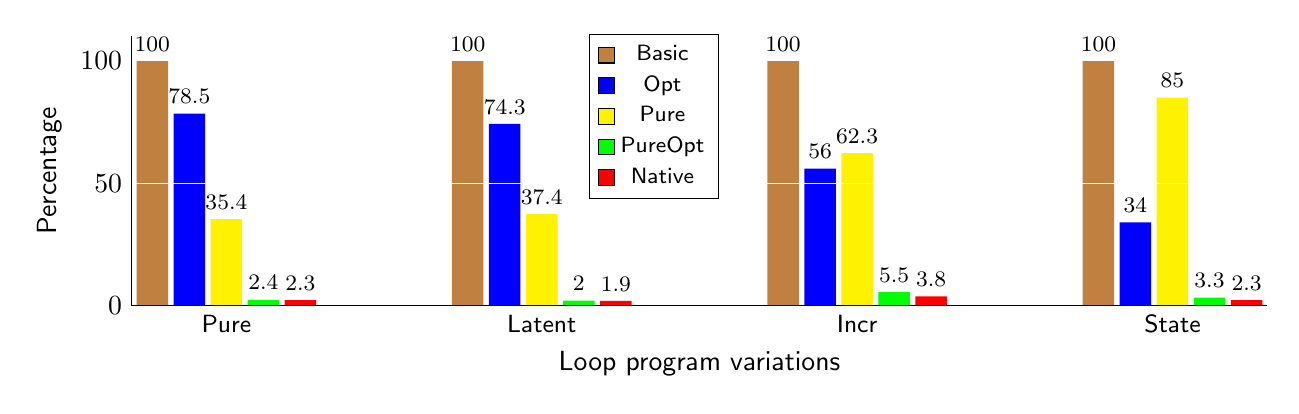
\begin{tikzpicture}
  \centering
  \begin{axis}[
        ybar, axis on top,
        height=5cm, width=16cm,
        ymajorgrids, tick align=inside,
        bar width=0.4cm,
        major grid style={draw=white},
        enlarge y limits={value=.1,upper},
        ymin=0, ymax=100,
        axis x line*=bottom,
        axis y line*=left,
        y axis line style={opacity=1},
        tickwidth=0pt,
        xtick = data,
        x tick label style={font=\small,text width=1.4cm,align=center},
         enlarge x limits=true,
      legend image code/.code={%
      \draw[#1] (0cm,-0.1cm) rectangle (0.2cm,0.1cm);
    },
            legend style={
            at={(0.46,1.01)},
            anchor=north,
            % legend columns=-1,
            % /tikz/every even column/.append style={column sep=0.4cm},
            font = \footnotesize
        },
        ylabel={Percentage},
        xlabel={Loop program variations},
           symbolic x coords={
           Pure,
           Latent,
           Incr,
           State,
           },
            nodes near coords={
         \footnotesize \pgfmathprintnumber{\pgfplotspointmeta}
        }
    ]
   \addplot [draw=none,fill=brown] coordinates {
      (Pure,100)
      (Latent,100)
      (Incr,100)
      (State,100)
       };

    \addplot [draw=none,fill=blue] coordinates {
      (Pure,78.5)
      (Latent,74.3)
      (Incr,56)
      (State,34)
      };

    \addplot [draw=none,fill=yellow] coordinates {
      (Pure,35.4)
      (Latent,37.4)
      (Incr,62.3)
      (State,85)
       };

    \addplot [draw=none,fill=green] coordinates {
      (Pure,2.4)
      (Latent,2)
      (Incr,5.5)
      (State,3.3)
       };

    \addplot [draw=none,fill=red] coordinates {
      (Pure,2.3)
      (Latent,1.9)
      (Incr,3.8)
      (State,2.3)
       }; 
   

    \legend{Basic, Opt, Pure, PureOpt, Native}
  \end{axis}
  \end{tikzpicture}
\caption{Relative run-times of Loops example  \cite{own}}
\label{fig:loops}
\end{figure}

\begin{figure}[H]
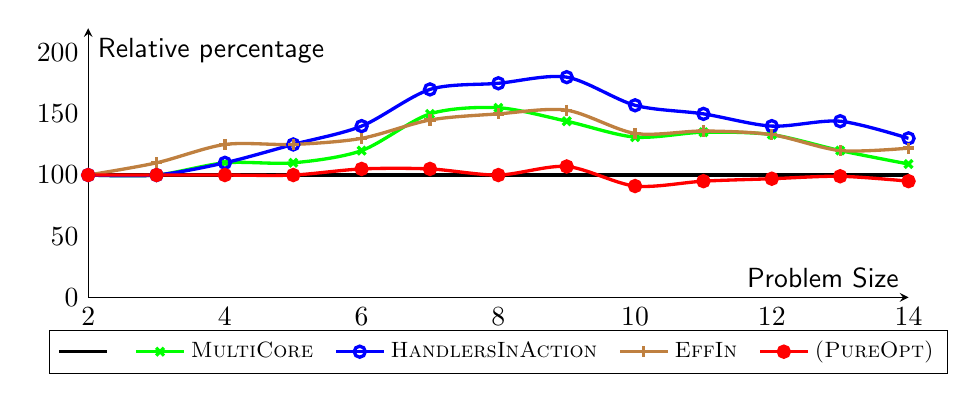
\begin{tikzpicture}
  \centering
  \begin{axis}[
        axis lines=center,
        axis on top,
        height=5cm, width=12cm,
        % bar width=0.4cm,
        % ymajorgrids, tick align=inside,
        major grid style={draw=white},
        enlarge y limits={value=.1,upper},
        ymin=0, ymax=200,
        axis x line*=bottom,
        axis y line*=left,
        % xtick = data,
        y axis line style={opacity=1},
        tickwidth=0pt,
        enlarge x limits=false,
        legend style={
            at={(0.5,-0.12)},
            anchor=north,
            legend columns=-1,
            /tikz/every even column/.append style={column sep=0.2cm},
            font = \footnotesize
        },
        ylabel={Relative percentage},
        xlabel={Problem Size},
           % symbolic x coords={
           % 0,
           % 8,
           % 9,
           % 10,
           % 11,
           % 12,
           % % 13,
           % % 14
           % },
       %      nodes near coords={
       %  \pgfmathprintnumber{\pgfplotspointmeta}
       % }
    ]
    %native
    \addplot [smooth,color = black, very thick] coordinates {
      (2,100)
      (3,100)
      (4,100)
      (5,100)
      (6,100)
      (7,100)
      (8,100)
      (9,100)
      (10,100)
      (11,100)
      (12,100)
      (13,100)
      (14,100)
       };
    %multicore
    \addplot [smooth,color = green, very thick, mark = x] coordinates {
      (2,100)
      (3,100)
      (4,110)
      (5,110)
      (6,120)
      (7,150)
      (8,155)
      (9,144)
      (10,131)
      (11,135)
      (12,133)
      (13,120)
      (14,109)
       };
    %HIA
   \addplot [smooth,color = blue, very thick, mark = o] coordinates {
      (2,100)
      (3,100)
      (4,110)
      (5,125)
      (6,140)
      (7,170)
      (8,175)
      (9,180)
      (10,157)
      (11,150)
      (12,140)
      (13,144)
      (14,130)
       };
    %EffectsinOcaml
   \addplot [smooth,color = brown, very thick, mark = +] coordinates {
      (2,100)
      (3,110)
      (4,125)
      (5,125)
      (6,130)
      (7,145)
      (8,150)
      (9,153)
      (10,134)
      (11,136)
      (12,133)
      (13,120)
      (14,122)
       };
    %PureOpt
   \addplot [smooth,color = red, very thick, mark = *] coordinates {
      (2,100)
      (3,100)
      (4,100)
      (5,100)
      (6,105)
      (7,105)
      (8,100)
      (9,107)
      (10,91)
      (11,95)
      (12,97)
      (13,99)
      (14,95)
       };

    \legend{\ocaml, \textsc{MultiCore}, \textsc{HandlersInAction}, \textsc{EffIn\ocaml}, \textsc{\eff}\textsc{(PureOpt)}}
  \end{axis}
  \end{tikzpicture}
\caption{Results of running N-Queens for all solutions on multiple systems  \cite{own}}
\label{fig:systemsall}
\end{figure}
\begin{figure}[H]
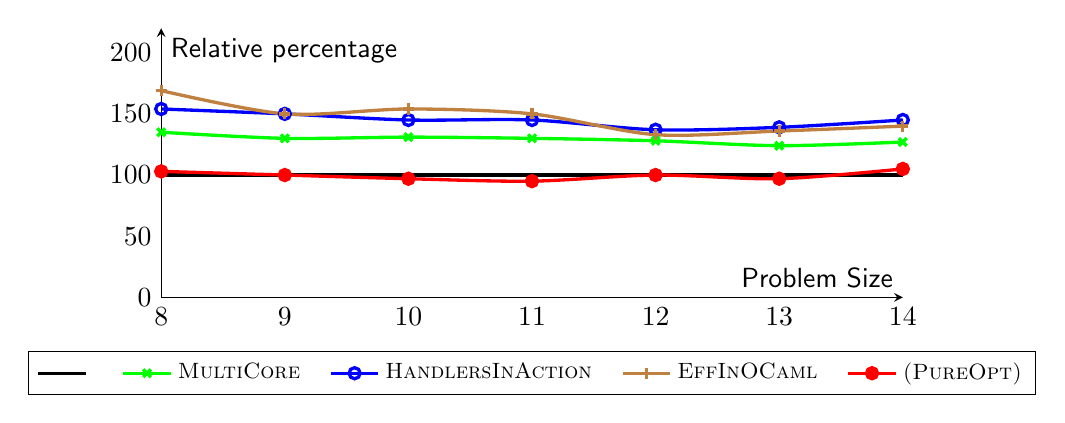
\begin{tikzpicture}
  \centering
  \begin{axis}[
        axis lines=center,
        axis on top,
        height=5cm, width=11cm,
        % bar width=0.4cm,
        % ymajorgrids, tick align=inside,
        major grid style={draw=white},
        enlarge y limits={value=.1,upper},
        ymin=0, ymax=200,
        axis x line*=bottom,
        axis y line*=left,
        xtick = data,
        y axis line style={opacity=1},
        tickwidth=0pt,
        enlarge x limits=false,
        legend style={
            at={(0.5,-0.2)},
            anchor=north,
            legend columns=-1,
            /tikz/every even column/.append style={column sep=0.3cm},
            font = \footnotesize
        },
        ylabel={Relative percentage},
        xlabel={Problem Size},
           % symbolic x coords={
           % 0,
           % 8,
           % 9,
           % 10,
           % 11,
           % 12,
           % % 13,
           % % 14
           % },
       %      nodes near coords={
       %  \pgfmathprintnumber{\pgfplotspointmeta}
       % }
    ]
    %native
    \addplot [smooth,color = black, very thick] coordinates {
      % (0,100)
      (8,100)
      (9,100)
      (10,100)
      (11,100)
      (12,100)
      (13,100)
      (14,100)
       };
    %multicore
    \addplot [smooth,color = green, very thick, mark = x] coordinates {
      (8,135)
      (9,130)
      (10,131)
      (11,130)
      (12,128)
      (13,124)
      (14,127)
       };
    %HIA
   \addplot [smooth,color = blue, very thick, mark = o] coordinates {
      (8,154)
      (9,150)
      (10,145)
      (11,145)
      (12,137)
      (13,139)
      (14,145)
       };
    %EffectsinOcaml
   \addplot [smooth,color = brown, very thick, mark = +] coordinates {
      (8,169)
      (9,150)
      (10,154)
      (11,150)
      (12,133)
      (13,136)
      (14,140)
       };
    %PureOpt
   \addplot [smooth,color = red, very thick, mark = *] coordinates {
      (8,103)
      (9,100)
      (10,97)
      (11,95)
      (12,100)
      (13,97)
      (14,105)
       };

    \legend{\ocaml, \textsc{MultiCore}, \textsc{HandlersInAction}, \textsc{EffInOCaml}, \textsc{\eff}\textsc{(PureOpt)}}
  \end{axis}
  \end{tikzpicture}
\caption{Results of running N-Queens for one solution on multiple systems  \cite{own}}
\label{fig:systemsone}
\end{figure}



\section{Reflection}
\input{reflection}

\section{Conclusions}
\input{conclusion}

\appendix
\input{zelfreflectie}
\section{Term rewriting: code}
\label{code}
Below is the code for the rule rewritting as implemented in the Eff compiler.
\begin{efflisting}[breaklines=true]
  | Handle ({term = Handler h}, c1)
        when (is_pure_for_handler c1 h.effect_clauses) ->
    useFuel st;
    (* Print.debug "Remove handler, since no effects in common with computation"; *)
    reduce_comp st (bind c1 h.value_clause)

  | Handle ({term = Handler h} as handler, {term = Bind (c1, {term = (p1, c2)})})
        when (is_pure_for_handler c1 h.effect_clauses) ->
    useFuel st;
    (* Print.debug "Remove handler of outer Bind, since no effects in common with computation"; *)
    reduce_comp st (bind (reduce_comp st c1) (abstraction p1 (reduce_comp st (handle (refresh_expr handler) c2))))

  | Handle ({term = Handler h}, {term = Bind (c1, {term = (p1, c2)})})
        when (is_pure_for_handler c2 h.effect_clauses) ->
    useFuel st;
    (* Print.debug "Move inner bind into the value case"; *)
    let new_value_clause = optimize_abs st (abstraction p1 (bind (reduce_comp st c2) (refresh_abs h.value_clause))) in
    let hdlr = handler {
      effect_clauses = h.effect_clauses;
      value_clause = refresh_abs new_value_clause;
    } in
    reduce_comp st (handle (refresh_expr hdlr) c1)

  | Handle ({term = Handler h} as h2, {term = Bind (c1, {term = (p, c2)})}) ->
    useFuel st;
    (* Print.debug "Move (dirty) inner bind into the value case"; *)
    let new_value_clause = optimize_abs st (abstraction p (handle (refresh_expr h2) (refresh_comp (reduce_comp st c2) ))) in
    let hdlr = handler {
      effect_clauses = h.effect_clauses;
      value_clause = refresh_abs new_value_clause;
    } in
    reduce_comp st (handle (refresh_expr hdlr) (refresh_comp c1))
    
  | Handle (h, {term = LetRec (defs, co)}) ->
  let handle_h_c = reduce_comp st (handle h co) in
  let res =
    let_rec' defs handle_h_c
  in
  reduce_comp st res
\end{efflisting}

\printbibliography

\end{document}